
\documentclass{beamer}


\usetheme{Frankfurt}
\usecolortheme{dove}
\usepackage{tikz}
\usetikzlibrary{arrows,shapes.arrows,positioning,shapes}
\usepackage{graphicx}
\usepackage{hyperref}
\newcommand\red[1]{{\color{red}#1}}
\newcommand\bred[1]{{\color{red}\textbf{#1}}}
\newcommand\blue[1]{{\color{blue}#1}}
\newcommand\bblue[1]{{\color{blue}\textbf{#1}}}
\newcommand\green[1]{{\color{olive}#1}}
\newcommand\bgreen[1]{{\color{olive}\textbf{#1}}}
\newcommand\black[1]{{\color{black}#1}}
\newcommand\white[1]{{\color{white}#1}}
\newcommand\gray[1]{{\color{darkgray}#1}}
\newcommand\E{\text{E}}
\newcommand\V{\text{V}}
\renewcommand\P{\text{P}}
\usepackage{soul}

\newcommand{\indep}{{\bot\negthickspace\negthickspace\bot}}

%%%%%%%%%%%%%%%%%%%%%%%%%%%%%%
\begin{document}

%\begin{frame}
%  \titlepage
%\end{frame}

\begin{frame}
\centering
\begin{tikzpicture}[x = .5\textwidth, y = .5\textheight]
\node[align = center, color = blue, font = \Large] at (0,.9) {Eviction among Children Born in Large U.S. Cities:\\\begin{large}Prevalence, Stratification, and Policy Levers\end{large}};
\node[align = center, font = \small] at (-.6, .52) {Ian Lundberg\\Princeton University};
\node[align = center, font = \footnotesize] at (0, .25) {12 August 2019\\Annual Meeting of the\\American Sociological Association};
\node[align = center, font = \footnotesize] at (.4,.52) {Joint work with Louis Donnelly, Sarah Gold,\\Sara McLanahan, and Jeanne Brooks-Gunn};
\node[align = left, font = \tiny] at (0,-.3) {\begin{minipage}{.9\textwidth}Slides and source code are available at \blue{\url{https://github.com/ilundberg/slides}}. We thank Sara S. McLanahan, Brandon M. Stewart, Matthew J. Salganik, Catherine Doren, three anonymous reviewers, and members of the Stewart Lab, Inequality Working Group, and Fragile Families Working Group for comments on earlier drafts. All errors are our own. Parts of this research were previously presented at APPAM 2018, PAA 2019, and a housing roundtable sponsored by the W.T. Grant Foundation at Princeton University. Research reported in this publication was supported by the Robert Wood Johnson Foundation and by The Eunice Kennedy Shriver National Institute of Child Health \& Human Development of the National Institutes of Health under Award Number P2CHD047879. Funding for the Fragile Families Study was provided through Award Numbers R01HD36916, R01HD39135, and R01HD40421 and by a consortium of private foundations. The content is solely the responsibility of the authors and does not necessarily represent the official views of the National Institutes of Health.\end{minipage}};
\end{tikzpicture}
\end{frame}

\section{Introduction}

\begin{frame}
Two claims in separate papers:
\begin{enumerate}
\item Eviction is \bblue{prevalent} and \bblue{stratified}
\item \only<1-1>{\bblue{Policy} can help}\only<2-3>{\textcolor{gray}{\textbf{Policy} can help}}
\end{enumerate} \vskip .5in
\onslide<3>{
(1) Published in \emph{Demography} [\href{https://link.springer.com/article/10.1007/s13524-018-0735-y}{\blue{link}}]

Replication code is on the Harvard Dataverse [\blue{\href{https://doi.org/10.7910/DVN/BVWFG1}{link}}].
}
\end{frame}

\begin{frame}
%Eviction is a \bblue{traumatic experience} for families. \pause \vskip .5cm
\begin{center}
\begin{tikzpicture}[x = 1in, y = .4in]
\node at (-1,-3) {};
\node at (1,3) {};
\node[anchor = west] at (-1,1.4) {Eviction may play a role in the \bblue{reproduction of poverty}.};
\node (poverty) at (0,0) {Poverty};
\node (eviction) at (1,0) {Eviction};
\node[align=center] (poverty2) at (2,0) {More\\poverty};
\only<1-1,3->{\draw[->, thick] (poverty) -- (eviction);}
\only<2-2>{\draw[->, blue, line width = 2pt] (poverty) -- (eviction);}
\only<2-2>{\node[darkgray] at (1, -2) {Desmond, Gershonson, \& Kiviat 2015};}
\draw[->, thick] (poverty) to[bend right] (poverty2);
\only<1-2,4->{\draw[->, thick] (eviction) -- (poverty2);}
\only<3-3>{\draw[->, blue, line width = 2pt] (eviction) -- (poverty2);}
\only<3-3>{\node[darkgray, align = center] at (1, -2) {Desmond \& Kimbro 2015\\Desmond \& Shollenberger 2015};}
\only<5->{\node[anchor = west] at (-1,-2) {Yet policymakers largely \bblue{ignore this problem.}};}
\end{tikzpicture}
\end{center}
\end{frame}

\section{Eviction is Prevalent}

\begin{frame}
Published studies suggest eviction is \bblue{rare in any given year}. \pause
\begin{itemize}
\item 0.3 \% of U.S. households in 12 months {\footnotesize \gray{(Bauman 2003)}} \pause
\item 2.3 \% in court records for 2016 {\footnotesize \gray{(Desmond et al. 2018)}} \pause
\end{itemize} \vskip .5cm
Eviction may be more common over the \bblue{course of childhood} \pause
\begin{itemize}
\item Families with children face a \bgreen{greater risk} {\footnotesize \gray{(Desmond et al. 2013)}} \pause
\item Risk \bgreen{accumulates} over time {\footnotesize \gray{(Duncan \& Rodgers 1988)}}
\end{itemize} \vskip .6cm \pause
\bblue{Research question:}
\begin{center}
What proportion of children born in large U.S. cities in 1998--2000\\
were \only<7-7>{ever evicted}\only<8-8>{\bgreen{ever evicted}} between birth and age 15?
\end{center}
%\begin{center}
%\begin{tabular}{rcccc}
%Bauman 2003 & 12 months in 1997--1998 & 0.3 \% \\
%Gould-Werth \& Seefeldt 2012 & 12 months in 2008--2010 in Detroit Metro Area &  2.4 \%
%%\end{tabular}
%\end{center}
\end{frame}

\begin{frame}
\includegraphics[width = \textwidth]{figures/ff_logo}
\begin{itemize}
\item Sampling frame: Births in 1998--2000 in U.S. cities with populations over 200,000
\item $N$ = 4,898 births in 20 cities
\begin{itemize}
\item 16 cities are a probability sample
\item 4 cities added for funder interests
\end{itemize}
\item Oversample (3:1) of non-marital births
\item Interviews with each parent at child age 1, 3, 5, 9, and 15
\end{itemize}
\end{frame}

\begin{frame}
\bblue{Survey instrument:}
\begin{center}
In the past 12 months, were you evicted from your home or apartment for not paying the rent or mortgage?
\end{center}
\begin{itemize}
\item[--] Reported by mother or father with whom child lives more than half the time
\end{itemize}
\end{frame}

\begin{frame}
\includegraphics[width = \textwidth]{figures/evByWave_weightedOnly}
\end{frame}

\begin{frame}
\centering
\begin{tikzpicture}[x = .5\textwidth, y = .5\textheight]
\node at (-1,-1) {};
\node at (1,1) {};
\node[anchor = west] at (-1, .7) {Child ages covered by eviction reports};
\node at (0,0) {\includegraphics[width = \textwidth]{figures/evictionData_largeLabels}};
% Block out parts of figure I will highlight in other ways on slide
\draw[color = white, fill = white] (-1,0.2) rectangle (1,.4);
\draw[color = white, fill = white] (-1,0.02) rectangle (0,.12);
\draw[color = white, fill = white] (-1,-.08) rectangle (1,-.03);
\only<2-2>{
	\node (annual) at (0, .23) {12 months preceding each survey};
	\draw[line width = 1.5pt, blue, rounded corners] (-.9,.07) rectangle (.95,.32);
}
\only<3-3>{
	\node[align = center] at (0.5, .5) {Retrospective:\\Any eviction between\\ages 9 and 15};
	\draw[->, line width = 1.5pt, blue] (0.5, 0.3) -- (0.5, 0.07);
}
\only<4-4>{
	\node[align = center] at (-.38, .5) {Periods with no report};
	\draw[->, line width = 1.5pt, blue] (-.07, 0.45) -- (-.07, 0.15);
	\draw[->, line width = 1.5pt, blue] (-.43, 0.45) -- (-.43, 0.15);
	\draw[->, line width = 1.5pt, blue] (-.67, 0.45) -- (-.67, 0.15);
}
\only<5-5>{
\node at (0,.5) {\bblue{Goal:} Proportion evicted at any point};
\draw[|-|, blue, line width = 2pt] (-.85,.4) -- (.9, .4);
}
\end{tikzpicture}
\end{frame}

\begin{frame}
\includegraphics[width = \textwidth]{figures/evictionModels_largeLabels}
\end{frame}

\section{Eviction is Stratified}

\begin{frame}
\centering \Large
Given our model, we can aggregate across the covariate values of specific \bblue{subgroups}.
\end{frame}

\begin{frame}
\includegraphics[width = \textwidth]{figures/RaceIncomeGroups_largeFont}
\end{frame}

\begin{frame}
\includegraphics[width = \textwidth]{figures/ByCity}
\end{frame}

\begin{frame}
Two claims in separate papers:
\begin{enumerate}
\item Eviction is \bblue{prevalent} and \bblue{stratified}
\item \bblue{Policy} can help
\end{enumerate}
\end{frame}

\section{Policy Can Help}

\begin{frame}
Two claims in separate papers:
\begin{enumerate}
\item \textcolor{gray}{Eviction is \textbf{prevalent} and \textbf{stratified}}
\item \bblue{Policy} can help
\end{enumerate}
\end{frame}

\begin{frame}{Research question}
\centering\large
Does \bblue{government assistance} protect\\low-income families from \bblue{eviction}? \vskip .6cm
\begin{tikzpicture}[x = .8\textwidth]
\node at (-.13, -4) {};
\node at (1.125, .8) {};
\onslide<2-5>{
\draw[|-, thick] (0,0) -- (9/15,0);
\node[anchor = south, align=center, font = \footnotesize] at (0,.1) {Age 0};
}
\onslide<6->{
\draw[|-, thick, gray] (0,0) -- (9/15,0);
\node[anchor = south, align=center, font = \footnotesize, gray] at (0,.1) {Age 0};
}
\onslide<2->{
\draw[|-|, thick] (9/15,0) -- (1,0);
\node[anchor = south, align=center, font = \footnotesize] at (9/15,.1) {Age 9};
\node[anchor = south, align=center, font = \footnotesize] at (1,.1) {Age 15};
}
\only<3-5>{
\node[anchor = north,align=center, font = \footnotesize] at (0,-.1) {Born 1998--2000\\large U.S. city};
}
\only<4-5>{
\node[anchor = north,align=center, font = \footnotesize, fill = white] at (9/15,0) {Resides with mother\\\\Family income\\below 200 \%\\federal poverty line\\\\Does not own home};
% for family of 4 (2 adults and 2 kids) that would be 51k in 2018
}
\onslide<7->{
\node[anchor = north, align=center, font = \footnotesize] at (9/15,-.1) {\bblue{Assistance}\\\bblue{received}};
}
\onslide<8->{
\node[anchor = north,align=center, font = \footnotesize, fill = white] at (12/15,-1) {\bblue{Ever}\\\bblue{evicted?}};
\draw[->, thick, blue] (12/15,-.9) -- (12/15,-.1);
}
\only<5>{
\node[anchor = south, align=center, font = \footnotesize] at (4.5/15,.1) {(control variables measured)};
}
\only<6->{
\node[anchor = south, align=center, font = \footnotesize] at (4.5/15,.1) {\textcolor{gray}{(control variables measured)}};
}
\end{tikzpicture} %\vskip .3cm
%For those residing in public housing,\\how much does assistance reduce $\P(\text{Eviction})$?
\end{frame}

\begin{frame}{Results}
\centering
\includegraphics[width = \textwidth]{figures/difference_estimators} \vskip 1in
\end{frame}

\begin{frame}
Two claims in separate papers:
\begin{enumerate}
\item Eviction is \bblue{prevalent} and \bblue{stratified}
\item \bblue{Policy} can help
\end{enumerate}
\end{frame}

\end{document}

\section{Limitations}

\begin{frame}{Limitations}
\begin{itemize}
\item Attrition may be non-ignorable \pause
\begin{itemize}
\item[$\rightarrow$] we will underestimate eviction
\end{itemize} \pause
\item Self-report may understate eviction \pause 
\begin{itemize}
\item[$\rightarrow$] we will underestimate eviction \pause
\end{itemize}
\item Parametric model may be wrong \pause
\begin{itemize}
\item[$\rightarrow$] implication unclear, but robust to random forest
\end{itemize}
\end{itemize}
\end{frame}

\begin{frame}
\centering
\begin{tikzpicture}[x = .5\textwidth, y = .5\textheight]
\node at (-1,-1) {};
\node at (1,1) {};
\node[font={\large\bf},blue,align=center] at (0,.8) {Government assistance protects low-income families\\from eviction and rent nonpayment};
\node (ian) at (-.65,0.5) {Ian Lundberg};
\node (sarah) at (0,0.5) {Sarah L. Gold};
\node (louis) at (.65,0.5) {Louis Donnelly};
\node (brooke) at (-.4,0.1) {Jeanne Brooks-Gunn};
\node (sara) at (.4,0.1) {Sara S. McLanahan};
\node[anchor = north, font = \tiny, align = center, outer sep = -4pt] at (ian.south) {Department of Sociology\\Office of Population Research\\Princeton University};
\node[anchor = north, font = \tiny, align = center, outer sep = -4pt] at (sarah.south) {Office of Population Research\\Princeton University};
\node[anchor = north, font = \tiny, align = center, outer sep = -4pt] at (louis.south) {Office of Population Research\\Center for Research on Child Wellbeing\\Princeton University};
\node[anchor = north, font = \tiny, align = center, outer sep = -4pt] at (brooke.south) {Teachers College\\College of Physicians and Surgeons\\Columbia University};
\node[anchor = north, font = \tiny, align = center, outer sep = -4pt] at (sara.south) {Department of Sociology\\Office of Population Research\\Center for Research on Child Wellbeing\\Princeton University};
\node[align=center] at (0,-.35) {Annual Meeting of the American Sociological Association\\12 August 2019};
\node[align=left, font = \tiny, text width = \textwidth] at (0,-.7) {We thank Catherine Doren, the Stewart Lab, the Inequality Working Group, and a housing roundtable sponsored by the W.T. Grant Foundation at Princeton University for helpful comments on earlier drafts. Research reported in this publication was supported by the Robert Wood Johnson Foundation and by The Eunice Kennedy Shriver National Institute of Child Health \& Human Development of the National Institutes of Health under Award Number P2CHD047879. Funding for the Fragile Families Study was provided through Award Numbers R01HD36916, R01HD39135, and R01HD40421 and by a consortium of private foundations. The content is solely the responsibility of the authors and does not necessarily represent the official views of the National Institutes of Health.};
\end{tikzpicture}
\end{frame}

\begin{frame}
\centering
\begin{tikzpicture}[x = .5\textwidth, y = .5\textheight]
\node[align = center, color = blue, font = \Large] at (0,.9) {A Research Note on the\\Prevalence of Housing Eviction\\Among Children Born in American Cities};
\node[align = center, font = \small] at (0, .52) {Ian Lundberg and Louis Donnelly\\Princeton University};
\node[align = center, font = \footnotesize] at (0, .25) {12 August 2019\\Annual Meeting of the\\American Sociological Association};
\node[align = left, font = \tiny] at (0,-.25) {\begin{minipage}{.9\textwidth}Slides and source code are available at \blue{\url{https://github.com/ilundberg/slides}}. Replication code is available on the Harvard Dataverse: \blue{\url{https://doi.org/10.7910/DVN/BVWFG1}}. Published in \emph{Demography} [\href{https://link.springer.com/article/10.1007/s13524-018-0735-y}{\blue{link}}]. Accepted manuscript is available \blue{\href{https://scholar.princeton.edu/sites/default/files/ilundberg/files/lundbergdonnelly2019_accepted.pdf}{here}}. We thank Sara S. McLanahan, Brandon M. Stewart, Matthew J. Salganik, three anonymous reviewers, and members of the Stewart Lab and the Fragile Families Working Group for comments on earlier drafts. All errors are our own. Research reported in this publication was supported by the Robert Wood Johnson Foundation and by The Eunice Kennedy Shriver National Institute of Child Health \& Human Development of the National Institutes of Health under Award Number P2CHD047879. Funding for the Fragile Families Study was provided through Award Numbers R01HD36916, R01HD39135, and R01HD40421 and by a consortium of private foundations. The content is solely the responsibility of the authors and does not necessarily represent the official views of the National Institutes of Health.\end{minipage}};
\end{tikzpicture}
\end{frame}